\subsection{Financial Statement Modelling}

\begin{definition} \hlt{Bottom-Up Analysis}\\
Begins with analysis if individual company of its reportable segments.\\
Revenue projects are based on historical revenue growth or company's new product introductions.\\
Another approach is through balance sheet composition forecasts (i.e., interest revenue forecasts for a bank) 
\end{definition}

\begin{definition} \hlt{Top-Down Analysis} \\
Begins with analysis on macroeconomic variable (expected growth rate of nominal GDP).\\
Forecasts then made at lower levels, such as sector, industry, and market for specific product, before arriving at a revenue projection for the individual company.
\end{definition}

\begin{definition} \hlt{Hybrid Analysis}\\
Incorporates both top-down and bottoms-up analysis.\\
May highlight any inconsistencies in assumptions between the two approaches.
\end{definition}

\begin{method} \hlt{Top-Down Approaches to Modelling Revenue}
\begin{enumerate}[label=\roman*.]
\setlength{\itemsep}{0pt}
\item Growth relative to GDP growth approach: relationship between GDP and company revenue is assumed to be at a rate of GDP growth rate times $1 + x\%$.
\item Market growth and market share approach: begin with estimate of industry sales (market growth), then company revenue is estimated as percentage of industry sales (market share). Market share times estimated industry sales provide estimate of company revenues.\\
Different business or geographic segments may have significantly different relationships between GDP growth and revenue growth.
\end{enumerate}
\end{method}

\begin{method} \hlt{Bottom-Up Approaches to Modelling Revenue}
\begin{enumerate}[label=\roman*.]
\setlength{\itemsep}{0pt}
\item Time series: forecasts based on historical growth rates or time-series analysis
\item Returns-based measure: based on BS accounts
\item Capacity-based measure: based on capacity of same-store sales growth and sales related to new stores.
\end{enumerate}
\end{method}

\subsubsection{Income Statement Modelling}

\begin{remark} \hlt{Economies of Scale on Operating Margins and Sales Levels}\\
Company with economies of scale will have lower average cost, hence higher operating margin.\\
Observed in larger companies that have higher sales.\\
To evaluate if company has economies of scale, look at common-size IS.\\
Economies of scale in COGS are evidenced by lower COGS as proportion of sales. Lower SG\&A as a proportion of sales is also evidence of economies of scale.
\end{remark}

\begin{remark} \hlt{Forecast of COGS}\\
As COGS is closely related to revenue, COGS is estimated as percentage of future revenue.
\begin{align}
\text{Forecast COGS} &= \frac{\text{Historical COGS}}{\text{Historical revenue}} \times \text{Forecast revenue} \nonumber \\
\text{Forecast COGS} &= (1 - \text{Gross margin}) \times \text{Forecast revenue} \nonumber
\end{align}
If company gross margin is on an increasing or decreasing trend (due to changes in business or market conditions), future gross margins should consider the probability of trend continuing.\\
To also cross check firm gross margin against competitors on if future gross margin estimates are reasonable.\\
More detailed analysis on volume and price improves quality of COGS forecast in the ST.\\
Firms with commodity as input cannot easily pass higher input costs to customers, hence will use hedging. To check for proportion of future input costs hedged this way, and if firm has historically hedged these costs. \\
COGS estimates improved by forecasting COGS for various product categories and business segments separately.
\end{remark}

\begin{remark} \hlt{Forecast of SG\&A Costs}\\
SG\&A costs are less sensitive to changes in sales volume as compared to COGS. \\
SG\&A fixed cost component is generally greater than its variable cost component. Expenses for salaries, IT operations etc. are more fixed than variable in nature, and grows as the firm grows.\\
R\&D expenditures are set by management and hence uncorrelated to revenues.\\
Selling and distribution costs are more correlated with sales volumes.\\
To break SG\&A component into different components and segments for better forecasts.
\end{remark}

\begin{remark} \hlt{Financing Cost Forecast}\\
Primary factors of gross interest payment are the level of (gross) debt and market interest rates.\\
Companies may also have interest income from payments, true for banks and other financial companies, and less so for non-financial companies such as manufacturers.
\begin{align}
\text{Net debt} &= \text{Gross debt} - \text{Cash, cash equivalents, other ST securities} \nonumber \\
\text{Net interest expense} &= \text{Gross interest expense} - \text{Interest income on cash and ST debt securities} \nonumber
\end{align}
Include planned debt issuance or retirement and maturity of structure of existing debt (disclosed in footnotes to financial statements) to improve forecasts of future financing costs.
\end{remark}

\begin{remark} \hlt{Types of Tax Rates}
\begin{enumerate}[label=\roman*.]
\setlength{\itemsep}{0pt}
\item Statutory rate: percentage tax charged in country where firm is domiciled
\item Effective tax rate: income tax expense as percentage of pretax income on IS
\item Cash tax rate: cash taxes paid as percentage of pretax income
\end{enumerate}
\end{remark}

\begin{remark} \hlt{Income Tax Expense Forecast}\\
Changes in deferred tax items account for difference between income tax expense and cash taxes due. Note,
\begin{equation}
\text{Income tax expense} = \text{Cash tax due} + (\Delta \text{Deferred tax liabilities} - \Delta \text{Deferred tax assets}) \nonumber
\end{equation}
Reconciliation of difference between statutory and effective tax rates is in footnotes to financial statements, and can provide information on one-time events, and tax rates for various jurisdictions in which the firm operates.\\
Statutory and effective tax rates may differ due to:
\begin{enumerate}[label=\roman*.]
\setlength{\itemsep}{0pt}
\item Expenses recognised in IS that are not deductible for tax purposes (permanent difference)
\item Company with higher (lower) earnings growth in high tax country will have higher effective tax rate.
\end{enumerate}
Pay attention to estimates of tax rates for companies that consistently report an effective tax rate less than statutory rate, or consistently less than that of comparable peer companies.
\end{remark}

\begin{remark} \hlt{Other Items Forecast}\\
Dividends estimated based on historical data, using constant growth rate, or constant payout ratio.\\
Forecast of number of shares outstanding due to share repurchases and issuances require analysts to pay attention to stated changes in capital structure.\\
Unusual charges to be excluded in forecasts. If company has history of such charges, then a normalised amount of such charges to be included in expense forecasts.
\end{remark}

\begin{figure}[H]
\centering
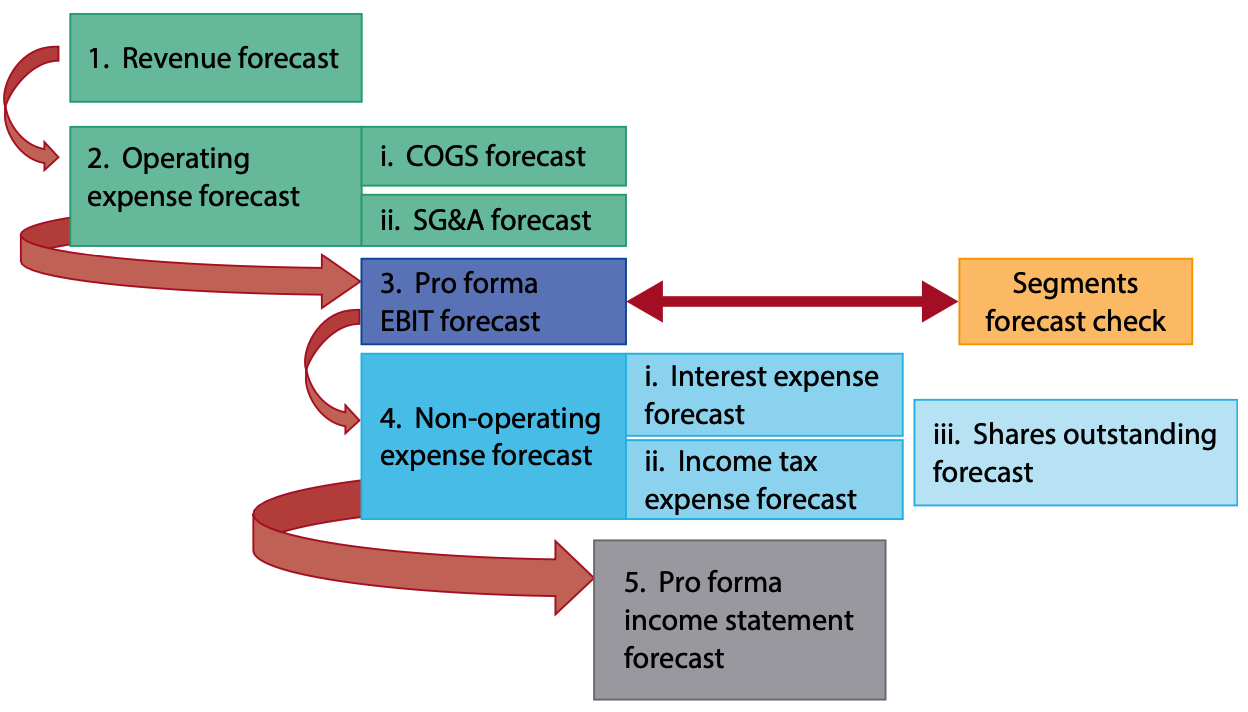
\includegraphics[scale=0.5]{fsa/isforecast}
\caption{Income statement forecast process}
\end{figure}

\subsubsection{Balance Sheet and Cash Flow Statement Modelling}

\begin{remark} \hlt{Balance Sheet Forecast}\\
Items from forecast IS flow into BS items
\begin{enumerate}[label=\roman*.]
\setlength{\itemsep}{0pt}
\item Net income less dividends from IS declared will flow to retained earnings
\item Working capital items can be forecasted based on historical relationship with IS items.
\item $\frac{\text{Forecasted annual COGS}}{\text{Inventory turnover ratio}}$ from IS can be used to forecast inventory value consistent with IS COGS projections
\item DSO from IS can be used to forecast
\begin{equation}
\text{Projected accounts receivables} = \text{DSO} \times \frac{\text{Forecasted sales}}{365} \nonumber
\end{equation}
Estimates derived this way will preserve working capital items relationship with IS items. Absent any complicating factors, working capital items will increase at same rate as revenues.
\item PPE on BS determined by depreciation and Capex. To estimate PPE, assume it will be equal to historical average proportion of sales, hence PPE will grow at same rate as revenue.
\item Forecasts may be improved by info on company's operations and future plans (hence forecast future capital needs), and by analysing Capex for maintenance separately from Capex for growth.
\item Historical depreciation to be increased by inflation rate when estimating Capex for maintenance as replacement costs can be expected to increase with inflation.
\end{enumerate}
\end{remark}

\begin{remark} \hlt{Post-Forecast Analysis of Balance Sheet}\\
Perform sensitivity analysis for individual assumptions, or with alternative assumptions (scenario analysis), to examine sensitivity of net income to changes in assumptions.
\end{remark}

\begin{figure}[H]
\centering
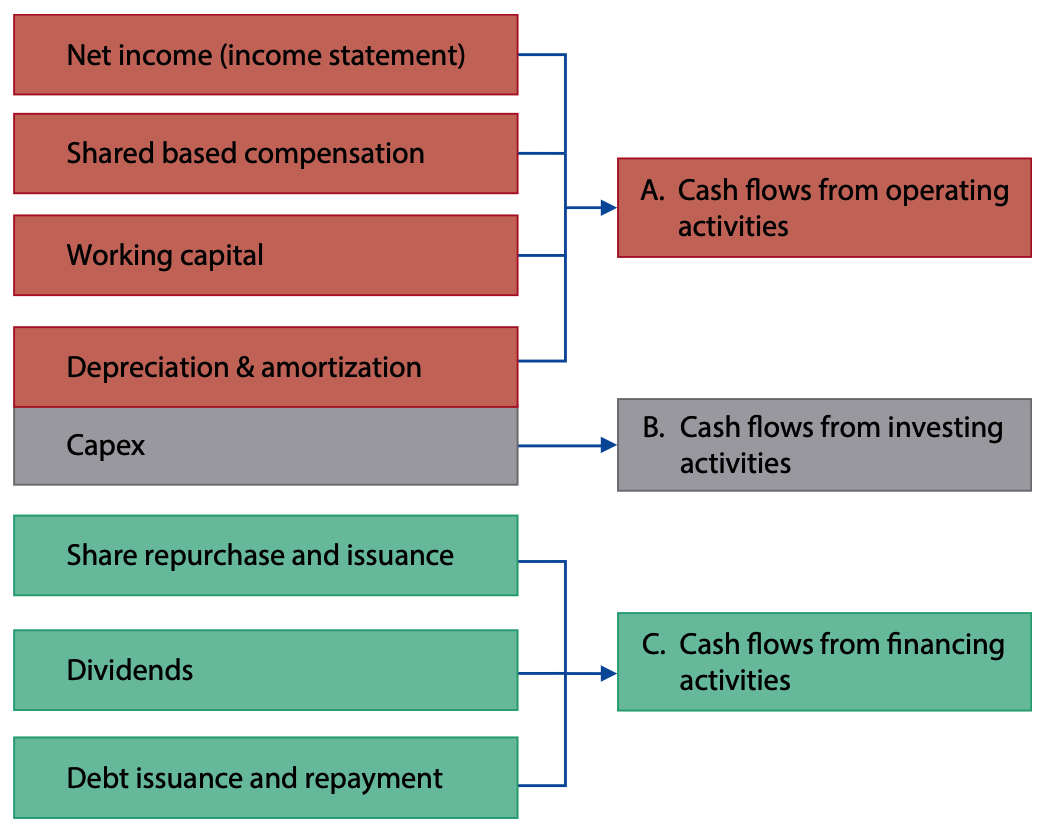
\includegraphics[scale=0.5]{fsa/cfsforecast}
\caption{Cash flow statement forecast process}
\end{figure}

\subsubsection{Behavioural Bias in Analysis Forecasts}

\begin{remark} \hlt{Overconfidence Bias}\\
Underestimation of forecast errors, hence a narrower confidence interval for forecasts than warranted.\\
Evaluate efficacy of past forecasts and learn from previous forecasting errors.\\
Scenario analysis may help identify shortcomings.
\end{remark}

\begin{remark} \hlt{Illusion of Control Bias}\\
False sense of security in one's forecast. Bias is manifested when:
\begin{enumerate}[label=\roman*.]
\setlength{\itemsep}{0pt}
\item expert opinion are used to justify a forecast
\item making a model more complex and granular (by adding more independent variables).
\end{enumerate}
Overfitted models perform poorly out of sample, conceal assumptions not updated based on new information.\\
Mitigated by focusing only on variables with known explanatory power, and by seeking outside opinions only from those with unique or specific perspective.
\end{remark}

\begin{remark} \hlt{Conservatism Bias (Anchoring)}\\
Only small adjustments are made to prior forecasts when new information becomes available.\\
Results in reluctance to incorporate new negative information, and lags in incorporating positive information.\\
Mitigation requires periodic evaluation of forecasting errors, using more parsimonious models.
\end{remark}

\begin{definition}
A phenomenon's rate of incidence in a larger population is the \hlt{base rate}.\\
Focus on base rate (viewing the company as member of particular industry) is the 'outside view', while situation-specific view (fixating on firm's company specific factors is the 'inside view'.
\end{definition}

\begin{remark} \hlt{Representativeness Bias}\\
Occurs due to tendency to classify data based on past information and known classifications.\\
New information may only be superficially similar to a known classification, hence best viewed from a fresh perspective. One common form of the bias is the base-rate neglect, where an observation's membership (its base rate) is neglected in favour of situation or member-specific information.\\
To consider both inside and outside view to generate forecasts.
\end{remark}

\begin{remark} \hlt{Confirmation Bias}\\
Causes analyst to seek out or pay attention to data that affirms their earlier convictions, and to disregard or underestimate information that disputes those opinions.\\
To reduce bias, keep abreast of research from analysts with opposite views, or seek out points of view from colleagues with no emotional investment.\\
To recognise inherent biases while evaluating management representations.
\end{remark}

\subsubsection{Competitive Analysis and Growth Rate}

\begin{definition} \hlt{Return on Invested Capital (ROIC)} \\
ROIC is a return on both equity and debt, allows comparisons across firms with different capital structures.
\begin{align}
\text{ROIC} &= \frac{\text{Net operating profit adjusted for taxes (NOPLAT)}}{\text{Invested capital}} \nonumber \\
\text{Invested capital} &= \text{Operating assets} - \text{Operating liabilities} \nonumber
\end{align}
Firms with higher ROIC relative to peers are likely exploiting some competitive advantage in production and/or sale of their products.
\end{definition}

\begin{remark} \hlt{Porter's Five Forces}\\
Industry characteristics may affect future financial results and financial forecasts.
\begin{enumerate}[label=\roman*.]
\setlength{\itemsep}{0pt}
\item Threat of substitute products: less pricing power when threat is high and switching costs are low
\item Intensity of industry rivalry: less pricing power when intensity is high. Pricing power is low when industry concentration is low, fixed costs and exit barriers are high, industry growth is slow or negative, products are not differentiated to a significant degree
\item Bargaining power of suppliers: prospects for earnings growth lower when bargaining power is high. If suppliers are few, able to extract a larger portion of any value added
\item Bargaining power of customers: less pricing power when bargaining power is high, when small number of customers are responsible for large proportion of firm's sales, and when switching costs are low
\item Threat of new entrants: more pricing power and better prospects for earnings growth when threat is low. Significant barriers to entry allows existing companies to maintain high returns on invested capital
\end{enumerate}
\end{remark}

\begin{remark} \hlt{Sales Projections with Inflation and Deflation}
\begin{enumerate}[label=\roman*.]
\setlength{\itemsep}{0pt}
\item Industry sales: most increases in costs (i.e., commodities or labour) will result in higher prices for end- products. Industry structure is important in determining the relationship between increases in input costs and increase in price of end products.\\
If demand is price elastic, company's effort to pass on inflation with higher prices can have negative impact on volume if cheaper substitutes are available. In inflationary environment, raising prices too late will squeeze profit margin, and acting too soon will result in volume loss. In deflationary environment, lowering prices too soon will result in lower price margin, waiting too long will result in volume loss.
\item Company sales: revenue projections are based on expected volume and price development.\\
Revenue forecast with inflation requires input of price elasticity of the products, different rates of cost inflation in active countries, and likely inflation in costs relevant to individual product categories.
\end{enumerate}
\end{remark}

\begin{remark} \hlt{Cost Projections with Inflation and Deflation}
\begin{enumerate}[label=\roman*.]
\setlength{\itemsep}{0pt}
\item Industry costs: inputs for modelling includes purchasing practices, expected input price fluctuations, use of long-term contracts or hedges. To monitor the underlying drivers of input prices as well.\\
Impact of inflation or deflation on industry cost structure depends on its competitive environment, i.e., if participants in industry have access to alternative inputs or are vertically integrated.
\item Company costs: segment cost structure by category and geography. For each item of cost, the assessment of impact on potential inflation and deflation in input prices should take into account company's ability to substitute cheaper alternative for expensive inputs, or increase efficiency to offset the impact of inflation.
\end{enumerate}
\end{remark}

\begin{remark} \hlt{Technological Developments}\\
Advanced in technology decreases cost of production; increase profit margin, industry supply and unit sales.\\
There may also be improved substitutes, or wholly new products, and markets and industries are disrupted.\\
To model introduction of new substitutes for company's products, estimate a cannibalisation factor:
\begin{equation}
\text{Cannibalisation rate} = \frac{\text{New product sales that replace existing product sales}}{\text{Total new product sales}} \nonumber
\end{equation}
The cannibalisation factor can be different for different sales channels, and is likely to be lower for business customers than for direct purchases by customers.\\
Use scenario and sensitivity analysis.
\end{remark}

\begin{remark} \hlt{Considerations in Choice of Explicit Forecast Horizon}\\
For buy-side analyst, appropriate forecast horizon may be expected holding period of stock, considered in conjunction with the investment strategy for the stock being considered.\\
Highly cyclical companies are difficult to model for long time horizons.\\
Horizon should be long enough to incorporate business cycles.\\
Normalised earnings are expected mid-cycle earnings, or cyclicality are no longer affecting earnings.\\
Corporate events such as M\&A, restructurings, should be considered temporary, and forecast benefits should be long enough that the perceived benefits of such events can be realised.
\end{remark}

\begin{remark} \hlt{Considerations in Developing Projections Beyond Short-Term Horizon}\\
Earnings projects beyond short-term assumed based on the trend growth rate of revenue over previous cycle.\\
Terminal value estimated using either relative valuation (i.e., price multiple), or DCF approach.\\
Ensure multiples used is consistent with estimate of company growth rate and required rate of return.\\
For DCF, inputs are CF or earnings measure and expected future growth rate. Expected earnings or CF to be normalised to mid-cycle value. Future growth rate to be modelled based on inflection points, which may occur due to changes in overall economic environment, business cycle stage, government regulations, and technology.
\end{remark}

\begin{method} \hlt{Steps in Development of Sales-Based Pro Forma Company Model}\\
To use segment information and create segment forecasts when company has business or geographical segments that differ from each other in important aspects. Use sensitivity analysis or scenario analysis to estimate range of possible outcomes and their possibilities.\\
Steps in developing the pro forma model is as follows:
\begin{enumerate}[label=\roman*.]
\setlength{\itemsep}{0pt}
\item Estimate revenue growth and future expected revenue (using market growth plus market share, trend growth rate, or growth relative to GDP growth)
\item Estimate COGS (based on percentage of sales, or based on business strategy, competitive environment)
\item Estimate SG\&A (as either fixed, growing with revenue, or other estimation technique)
\item Estimate financing costs (with interest rates, debt levels, effects of any large anticipated changes in capital expenditures or anticipated changes in financial structure)
\item Estimate income tax expense and cash taxes (using historical effective rates and trends, segment information for different tax jurisdictions, and anticipated growth in high- and low-tax segments)
\item Estimate cash taxes, taking into account changes in deferred tax items
\item Model the BS based on items that flow from IS (working capital accounts, i.e., accounts receivable, accounts payable, and inventory)
\item Use depreciation and capital expenditures (for maintenance and for growth) to estimate capital expenditures and net PPE for the BS
\item Use completed pro forma IS and BS to construct pro forma CFS
\end{enumerate}
Estimation methods ca be simple or more complex. To decide on when an additional or more complex analysis is warranted, and when additional complexity in estimation method provides real benefits to forecasts.
\end{method}
